\documentclass{article}
\usepackage{tikz}
\pagestyle{empty}
%---------------------------------
\begin{document}

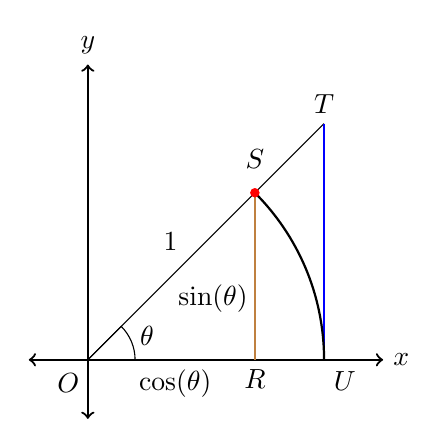
\begin{tikzpicture}[scale=3]
\draw (0,0) -- (2mm,0mm) arc (0:45:2mm) -- cycle; %angle arc for the triangle
\draw[<->, thick] (-.25,0) -- (1.25,0) node[right]{$x$}; %x-axis and it's label
\draw[<->, thick] (0,-.25) -- (0,1.25) node[above]{$y$}; %y-axis and it's label
\draw (0,0) -- (1,1); %line from origin to (1,1)
\draw[thick, brown] (.7071,0) -- (.7071,.7071); %brown line 
\draw[thick, blue] (1,0)--(1,1);   % blue line
\begin{scope} %draws that part of the circle that is contained in the rectangle
\clip (.5,0) rectangle (1.1,.71);
\draw[black, thick] (0,0) circle (1cm); %The circle
\end{scope}

\filldraw[red] (.7071,.7071) circle (.5pt); %the red dot at point (x,y)
\draw (.25,.1) node {$\theta$}; %label the angle theta
\draw (.35,.5) node {$1$}; % label of the radius
\draw (.7071,.77) node[above] {$S$}; %label M
\draw (1,1) node[above] {$T$}; %label M
\draw (.37,0) node[below] {$\cos(\theta)$}; %cos(theta) label
\draw (.53,.36) node[below] {$\sin(\theta)$}; %sin(theta) label
\draw (.7071,.0) node[below] {$R$}; % R label
\draw (1,-.09) node[below,right] {$U$}; % U label
\draw (-.17,-.1) node[below,right] {$O$}; % O label
\end{tikzpicture}

\end{document}


